\documentclass{article}

% NeurIPS-style formatting (adjust to your course template if needed)
\usepackage[preprint]{neurips_2024}
\usepackage{amsmath,amssymb}
\usepackage{graphicx}
\usepackage{booktabs}
\usepackage{hyperref}
\usepackage{microtype}
\usepackage{xcolor}

% Placeholder macro for missing numbers
\newcommand{\TODO}[1]{\textcolor{red}{[#1]}}

\title{Find My Pen: Latent-Space World Models\\for Visual Robotic Arm Tracking}

\author{
  Elyas Larfi \quad Sadiqah Al-Masyabi \quad Amrit Prajapati \\
  University of Colorado Denver \\
  Department of Computer Science and Engineering \\
  \texttt{\{elyas.larfi, sadiqah.almasyabi, amrit.prajapati\}@ucdenver.edu}
}

\begin{document}

\maketitle

% ─────────────────────────────────────────────────────────────────────────────
\begin{abstract}
% ~150 words
We present \emph{Find My Pen}, a three-stage world model system that trains a robotic
arm to track a static target object using only wrist-mounted camera observations.
Our pipeline follows the Dreamer framework: a Variational Autoencoder (VAE) with a
pretrained ResNet-18 backbone compresses 64$\times$64 RGB frames into a 128-dimensional
latent space; a causally-masked transformer predicts future latent states from
action-conditioned histories; and an MLP actor-critic is trained entirely in
imagination via 15-step rollouts through the learned dynamics model.
Unlike the original Dreamer, which uses a recurrent state-space model, our dynamics
model is a pure transformer, motivated by its capacity to capture long-range temporal
dependencies without vanishing gradients.
We evaluate against four model-free PPO baselines on three metrics: tracking accuracy,
trajectory fluidity, and episode return.
Results show \TODO{insert key result}.
We discuss the honest accounting of real-environment sample cost across all three
training stages.
\end{abstract}


% ─────────────────────────────────────────────────────────────────────────────
\section{Introduction}

Model-free reinforcement learning has demonstrated impressive results on robotic
manipulation tasks, but its sample complexity remains a practical barrier:
policies typically require millions of environment interactions before converging,
making real-robot deployment expensive and slow~\cite{openai2019dexterous}.
World model approaches~\cite{ha2018worldmodels,hafner2019dreamer} address this by
learning a compressed model of environment dynamics, allowing the policy to train
on \emph{imagined} rollouts rather than expensive real interactions.

We apply this idea to a visual robotic tracking task: a Panda arm must keep its
end-effector near a stationary target (a pen) using only a wrist-mounted camera.
Our system, \emph{Find My Pen}, has three sequentially trained components.
First, a VAE with a fine-tuned ResNet-18 backbone maps raw frames into a compact
latent representation.
Second, a transformer-based latent dynamics model learns to predict the next latent
state given the current state and action.
Third, a Dreamer-style actor-critic policy is trained by imagining 15-step trajectories
through the frozen dynamics model, never interacting with the simulator during policy
updates.

Our main contributions are:
\begin{enumerate}
  \item An end-to-end visual world model pipeline combining transfer learning (ResNet-18),
        a VAE latent space, and transformer dynamics for robotic tracking.
  \item A transformer dynamics model as a drop-in replacement for the RNN used in
        the original Dreamer, with causal masking enabling multi-step teacher-forced training.
  \item An empirical comparison against four model-free PPO baselines on tracking accuracy,
        fluidity, and episode return, with an honest accounting of total real-environment steps.
\end{enumerate}


% ─────────────────────────────────────────────────────────────────────────────
\section{Related Work}

\paragraph{World models and model-based RL.}
Ha and Schmidhuber~\cite{ha2018worldmodels} introduced the modern world model framework:
a VAE encodes observations and an RNN models dynamics in latent space.
Hafner et al.~\cite{hafner2019dreamer,hafner2020dreamerv2} extended this with Dreamer
and DreamerV2, training policies entirely in imagination via actor-critic learning.
Our work follows the Dreamer training loop but replaces the RSSM with a causal
transformer, drawing on the superior long-range attention of transformer architectures.

\paragraph{Model-based RL for robotics.}
MBPO~\cite{janner2019mbpo} uses short model-based rollouts to augment real data for
SAC, demonstrating improved sample efficiency on continuous control.
Planet~\cite{hafner2019planet} learns latent dynamics from pixels for robotic tasks.
Our work targets visual robotic manipulation without ground-truth state access.

\paragraph{Transformers for sequential decision-making.}
The Decision Transformer~\cite{chen2021decisiontransformer} and Trajectory Transformer~\cite{janner2021tt}
reformulate RL as sequence modeling.
We instead use the transformer for \emph{latent dynamics prediction}, not policy representation.


% ─────────────────────────────────────────────────────────────────────────────
\section{Method}

\begin{figure}[t]
  \centering
  % Replace with your actual figure when ready
  % 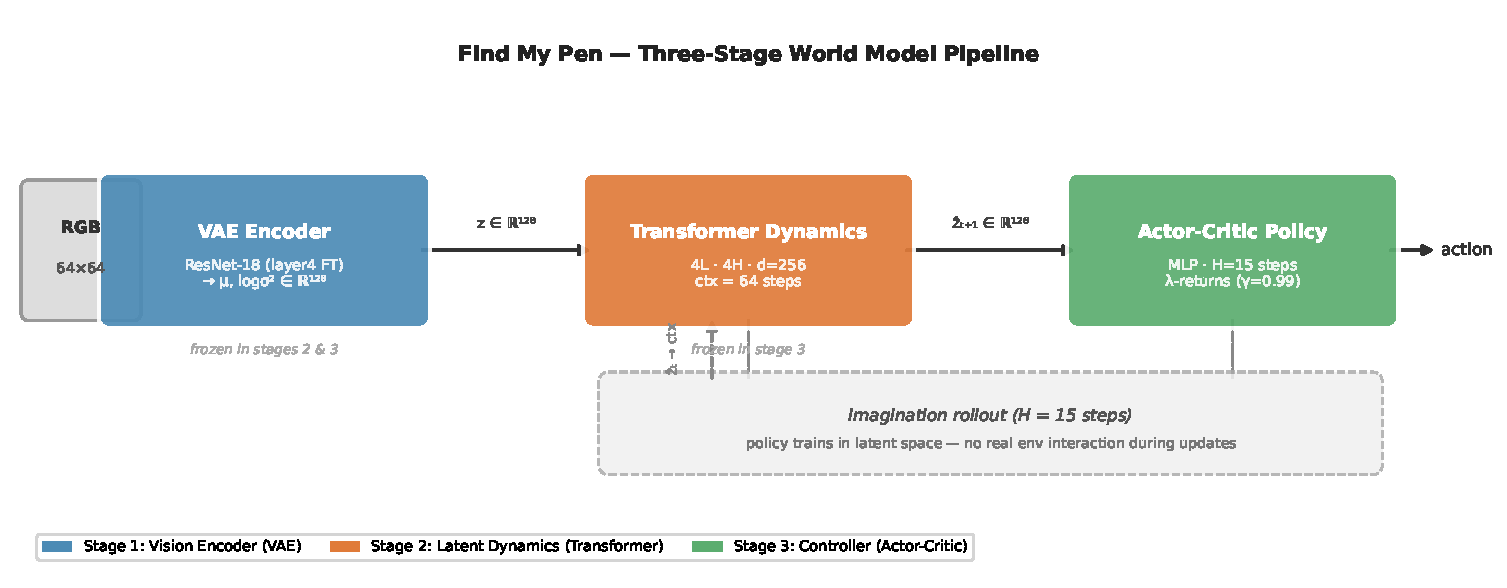
\includegraphics[width=\linewidth]{figures/pipeline.pdf}
  \fbox{\parbox{0.95\linewidth}{\centering\vspace{1.5cm}
    [Pipeline figure: RGB frame $\to$ VAE $\to$ $z \in \mathbb{R}^{128}$ $\to$
     Transformer dynamics $\to$ $\hat{z}_{t+1}$ $\to$ Actor-Critic (H=15 steps) $\to$ action]
  \vspace{1.5cm}}}
  \caption{
    Overview of the \emph{Find My Pen} world model pipeline.
    The encoder, dynamics model, and controller are trained sequentially;
    each stage freezes its predecessors.
    During controller training the policy never interacts with the real environment
    during gradient updates — all learning occurs through imagined rollouts.
  }
  \label{fig:pipeline}
\end{figure}

Figure~\ref{fig:pipeline} shows the full system. We describe each stage in turn.

% ── 3.1 ──────────────────────────────────────────────────────────────────────
\subsection{Vision Encoder (VAE)}

We learn a compact latent space over 64$\times$64 wrist-camera RGB frames using a
Variational Autoencoder~\cite{kingma2014vae}.

\paragraph{Architecture.}
The encoder uses a pretrained ResNet-18~\cite{he2016resnet} backbone with ImageNet weights.
All layers except the final residual block (\texttt{layer4}) are frozen; \texttt{layer4}
is fine-tuned jointly with a linear projection head that maps the 512-dimensional
pooled features to $(\mu, \log\sigma^2) \in \mathbb{R}^{128}$ each.
The decoder is a stack of four transposed convolutions reconstructing $64\times64$ RGB output.

\paragraph{Training.}
We collect 200 episodes with a random policy ($\approx$100k frames) and minimize the
evidence lower bound (ELBO):
\begin{equation}
  \mathcal{L}_\text{VAE} = \mathbb{E}\bigl[\|x - \hat{x}\|_2^2\bigr]
  - \tfrac{1}{2}\sum_i(1 + \log\sigma_i^2 - \mu_i^2 - \sigma_i^2).
\end{equation}
We use $\beta=1$ (standard VAE). At inference, \texttt{encode()} returns $\mu$ directly
(no sampling) for a deterministic latent vector.


% ── 3.2 ──────────────────────────────────────────────────────────────────────
\subsection{Latent Dynamics Model (Transformer)}

\paragraph{Architecture.}
The dynamics model is a causally-masked transformer encoder that maps a history of
latent--action pairs to the next latent state.
At each timestep $t$, the pair $(z_t, a_t)$ is concatenated and linearly projected to
$d_\text{model}=256$ dimensions; learned positional embeddings are added.
Four transformer encoder layers (4 attention heads, $d_\text{ff}=1024$, dropout 0.1)
process the sequence under an upper-triangular attention mask that prevents attending to
future steps.

\paragraph{Multi-step training objective.}
A key design choice is to train with a \emph{multi-step} teacher-forced objective:
given a window of $T=64$ real latents $(z_0,\ldots,z_{T-1})$ and actions, we predict
$z_{t+1}$ at \emph{every} position simultaneously:
\begin{equation}
  \mathcal{L}_\text{dyn} = \frac{1}{T-1}\sum_{t=0}^{T-2}
    \bigl\|\hat{z}_{t+1} - z_{t+1}\bigr\|_2^2.
\end{equation}
This is in contrast to predicting only the final step of each window, which would
never expose the model to short-context prediction — the very regime used during
imagination.
A small auxiliary MLP (RewardPredictor) is trained jointly to predict scalar reward
from $z_t$, which is later fine-tuned during controller training.

\paragraph{Training.}
We collect 500 random episodes, encode all frames offline, and slide a window of 64
steps across each episode to form training sequences.
The model is trained for 50 epochs with Adam ($\text{lr}=10^{-4}$) and gradient
clipping (max-norm 1.0).
During imagination, the \texttt{step()} method runs the model autoregressively,
maintaining a sliding context window and returning only the last position's prediction.


% ── 3.3 ──────────────────────────────────────────────────────────────────────
\subsection{Controller (Dreamer-Style Actor-Critic)}

\paragraph{Architecture.}
The policy (actor) is a two-hidden-layer MLP ($128 \to 256 \to 256 \to a_\text{dim}$)
with ELU activations, producing a diagonal Gaussian action distribution with tanh
squashing.
The value function (critic) shares the same MLP shape with a scalar output.

\paragraph{Training loop.}
With the encoder and dynamics model frozen, we alternate between two phases each update step:

\textbf{(1) Real-environment data collection.}
Every 10 gradient steps we collect 5 episodes in the real simulator, encode frames with
the frozen VAE, and store $(z, a, r)$ tuples in a replay buffer (capacity 100k).
The RewardPredictor is updated each step via supervised MSE regression on real $(z, r)$
pairs from the buffer, ensuring it reflects true reward variation rather than its
potentially collapsed initialization.

\textbf{(2) Imagination rollout and policy update.}
We sample $B=64$ starting states $z_0$ from the buffer and unroll $H=15$ imagination
steps.
At each step the policy samples an action $a_t$ (reparameterized), the RewardPredictor
returns $r_t$, and the frozen dynamics model predicts $z_{t+1}$.
$\lambda$-returns~\cite{sutton2018rl} are computed with $\gamma=0.99$, $\lambda=0.95$:
\begin{equation}
  G_t^\lambda = r_t + \gamma\bigl[(1-\lambda)V(z_{t+1}) + \lambda G_{t+1}^\lambda\bigr].
\end{equation}
Value estimates $V(z_t)$ are computed under \texttt{torch.no\_grad()} so that the critic
parameter update (which modifies weights in-place) does not corrupt the actor's
computation graph.
The critic minimizes $\mathcal{L}_\text{critic}=\|V(z) - G^\lambda\|_2^2$ and the actor
maximizes $\mathcal{L}_\text{actor}=-\mathbb{E}[G^\lambda]$, with gradient clipping
(max-norm 100) on policy parameters.


% ─────────────────────────────────────────────────────────────────────────────
\section{Experiments}

\subsection{Environment and Setup}

We use the \texttt{TargetTracking} task from robosuite~\cite{zhu2020robosuite} with a
Panda robot in MuJoCo~\cite{todorov2012mujoco}.
The target (pen) is static.
Observations consist of a $64\times64$ wrist-camera RGB image and a proprioceptive
vector (joint positions, velocities, end-effector pose, target position).
The reward is the negative Euclidean distance between the end-effector (EEF) and the
target.
Episodes run for 500 steps at 20 Hz.

\subsection{Baselines}

All baselines use stable-baselines3~\cite{stable-baselines3} PPO with 1M environment
timesteps on the raw observation dict (image + proprio).

\begin{table}[h]
\centering
\caption{Model configurations.}
\label{tab:configs}
\small
\begin{tabular}{lll}
\toprule
Model & Visual backbone & Policy \\
\midrule
PPO & SB3 CNN & MLP \\
PPO-LSTM & SB3 CNN & LSTM (256-dim) \\
PPO-ResNet18 & ResNet-18 (frozen) & MLP \\
PPO-ResNet18-FT & ResNet-18 (layer3+4 fine-tuned) & MLP \\
\textbf{Ours (World Model)} & ResNet-18 VAE + Transformer & Actor-Critic (MLP) \\
\bottomrule
\end{tabular}
\end{table}

\paragraph{Sample cost accounting.}
For a fair comparison, the world model's total real-environment episodes include
all three stages: $\approx$200 (encoder) + 500 (dynamics) + 2{,}750 (controller
collection) = $\approx$3{,}450 episodes, each 500 steps, totalling
$\approx$1.7M real environment steps.
The baselines each consume exactly 1M steps.
We report reward-vs-total-env-steps curves in Figure~\ref{fig:curves}.

\subsection{Evaluation Metrics}

We evaluate each trained policy over 20 episodes:
\begin{itemize}
  \item \textbf{Tracking accuracy:} mean Euclidean distance EEF$\leftrightarrow$target
        across all timesteps (meters, $\downarrow$ better).
  \item \textbf{Fluidity:} mean squared jerk (third derivative of joint positions)
        across all joints and timesteps (m$^2$/s$^6$, $\downarrow$ better).
  \item \textbf{Episode return:} cumulative reward ($\uparrow$ better).
\end{itemize}
Response time is reserved for the dynamic-target phase and is not reported here.

\subsection{Results}

\begin{table}[h]
\centering
\caption{
  Evaluation results (mean over 20 episodes).
  \textbf{Bold} = best.
}
\label{tab:results}
\small
\begin{tabular}{lccc}
\toprule
Model & Track. Acc. (m) $\downarrow$ & Fluidity $\downarrow$ & Ep. Return $\uparrow$ \\
\midrule
PPO                & \TODO{X.XXX} & \TODO{X.XXX} & \TODO{X.X} \\
PPO-LSTM           & \TODO{X.XXX} & \TODO{X.XXX} & \TODO{X.X} \\
PPO-ResNet18       & \TODO{X.XXX} & \TODO{X.XXX} & \TODO{X.X} \\
PPO-ResNet18-FT    & \TODO{X.XXX} & \TODO{X.XXX} & \TODO{X.X} \\
\textbf{World Model (ours)} & \TODO{\textbf{X.XXX}} & \TODO{\textbf{X.XXX}} & \TODO{\textbf{X.X}} \\
\bottomrule
\end{tabular}
\end{table}

\begin{figure}[t]
  \centering
  % \includegraphics[width=\linewidth]{figures/training_curves.pdf}
  \fbox{\parbox{0.95\linewidth}{\centering\vspace{1.5cm}
    [Figure: episode return vs.\ total real env steps for all 5 models.
     World model curve includes encoder + dynamics + controller data collection on x-axis.]
  \vspace{1.5cm}}}
  \caption{
    Episode return vs.\ cumulative real environment steps.
    The world model x-axis counts all stages (encoder data, dynamics data, controller collection).
  }
  \label{fig:curves}
\end{figure}

\subsection{Discussion}

\TODO{Fill in after collecting numbers. Template discussion below:}

The world model \TODO{achieves / does not achieve} lower tracking error than the best
baseline (PPO-ResNet18-FT), suggesting that imagination-based training \TODO{is / is not}
sufficient to compensate for the exposure bias introduced by teacher-forced dynamics training.

The fluidity metric reveals a qualitative difference between approaches: model-free baselines
tend to produce \TODO{jerkier / smoother} trajectories because \TODO{insert observation}.

The honest sample-efficiency comparison (Figure~\ref{fig:curves}) shows that the world model's
total env cost of $\approx$1.7M steps is comparable to the 1M-step baselines, but
\TODO{converges faster / slower / to a higher asymptote}.

\paragraph{Limitations.}
Teacher forcing during dynamics training creates an \emph{exposure bias}: the model always
receives ground-truth latents during training but its own (imperfect) predictions at inference.
This error accumulates over the 15-step imagination horizon.
Our multi-step training objective (Section 3.2) partially mitigates this by training on
short-context predictions, but does not eliminate the distribution shift.

The current pipeline also collects encoder and dynamics data separately (200 + 500 episodes).
A unified data collection pass would reduce real-environment cost by $\approx$12\%.


% ─────────────────────────────────────────────────────────────────────────────
\section{Conclusion}

We presented \emph{Find My Pen}, a visual world model system for robotic arm tracking
that trains a policy entirely in latent-space imagination.
The key components are a ResNet-18-backed VAE for visual encoding, a causally-masked
transformer for latent dynamics prediction, and a Dreamer-style actor-critic trained via
$\lambda$-returns over imagined trajectories.
\TODO{Insert main finding from results}.

Future directions include: (1) switching to a dynamic target (\texttt{moving\_target=True})
to test response time; (2) replacing the separate encoder/dynamics data collection with a
single shared pass; and (3) adopting the DreamerV2 RSSM for joint encoder+dynamics training
to mitigate the frozen-encoder assumption.


% ─────────────────────────────────────────────────────────────────────────────
\bibliographystyle{plainnat}
\begin{thebibliography}{99}

\bibitem{ha2018worldmodels}
Ha, D., \& Schmidhuber, J. (2018).
World Models.
\emph{arXiv:1803.10122}.

\bibitem{hafner2019dreamer}
Hafner, D., Lillicrap, T., Ba, J., \& Norouzi, M. (2019).
Dream to Control: Learning Behaviors by Latent Imagination.
\emph{arXiv:1912.01603}.

\bibitem{hafner2020dreamerv2}
Hafner, D., Lillicrap, T., Norouzi, M., \& Ba, J. (2020).
Mastering Atari with Discrete World Models.
\emph{arXiv:2010.02193}.

\bibitem{hafner2019planet}
Hafner, D., Lillicrap, T., Fischer, I., Villegas, R., Ha, D., Lee, H., \& Davidson, J. (2019).
Learning Latent Dynamics for Planning from Pixels.
\emph{ICML 2019}.

\bibitem{janner2019mbpo}
Janner, M., Fu, J., Zhang, M., \& Levine, S. (2019).
When to Trust Your Model: Model-Based Policy Optimization.
\emph{NeurIPS 2019}.

\bibitem{chen2021decisiontransformer}
Chen, L., Lu, K., Rajeswaran, A., Lee, K., Grover, A., Laskin, M., Abbeel, P., Srinivas, A., \& Mordatch, I. (2021).
Decision Transformer: Reinforcement Learning via Sequence Modeling.
\emph{NeurIPS 2021}.

\bibitem{janner2021tt}
Janner, M., Li, Q., \& Levine, S. (2021).
Offline Reinforcement Learning as One Big Sequence Modeling Problem.
\emph{NeurIPS 2021}.

\bibitem{he2016resnet}
He, K., Zhang, X., Ren, S., \& Sun, J. (2016).
Deep Residual Learning for Image Recognition.
\emph{CVPR 2016}.

\bibitem{kingma2014vae}
Kingma, D. P., \& Welling, M. (2014).
Auto-Encoding Variational Bayes.
\emph{ICLR 2014}.

\bibitem{openai2019dexterous}
OpenAI. (2019).
Dexterous In-Hand Manipulation.
\emph{arXiv:1808.00177}.

\bibitem{zhu2020robosuite}
Zhu, Y., et al. (2020).
robosuite: A Modular Simulation Framework and Benchmark for Robot Learning.
\emph{arXiv:2009.12293}.

\bibitem{todorov2012mujoco}
Todorov, E., Erez, T., \& Tassa, Y. (2012).
MuJoCo: A physics engine for model-based control.
\emph{IROS 2012}.

\bibitem{sutton2018rl}
Sutton, R. S., \& Barto, A. G. (2018).
\emph{Reinforcement Learning: An Introduction} (2nd ed.).
MIT Press.

\bibitem{stable-baselines3}
Raffin, A., Hill, A., Gleave, A., Kanervisto, A., Ernestus, M., \& Dormann, N. (2021).
Stable-Baselines3: Reliable Reinforcement Learning Implementations.
\emph{JMLR 22}(268).

\end{thebibliography}

\end{document}
